\chapter{Quantum Chromodynamics at the Large Hadron Collider}
\label{ch:qcd}

% ---------------------------------------------------------------
% WRITING NOTES:
%   Target: ~8–12 pages (Week 2: Mar 21–28)
%   Scope: do NOT rehash all of the SM.  Assume the reader knows
%          QED, electroweak theory, the Higgs mechanism.  Focus
%          entirely on the QCD aspects relevant to jet substructure
%          and the Z+jets measurement.
% ---------------------------------------------------------------

% ---------------------------------------------------------------
% Brief preamble: SM as the scaffolding, QCD as the focus
% ---------------------------------------------------------------

\begin{figure}[ht]
  \centering
  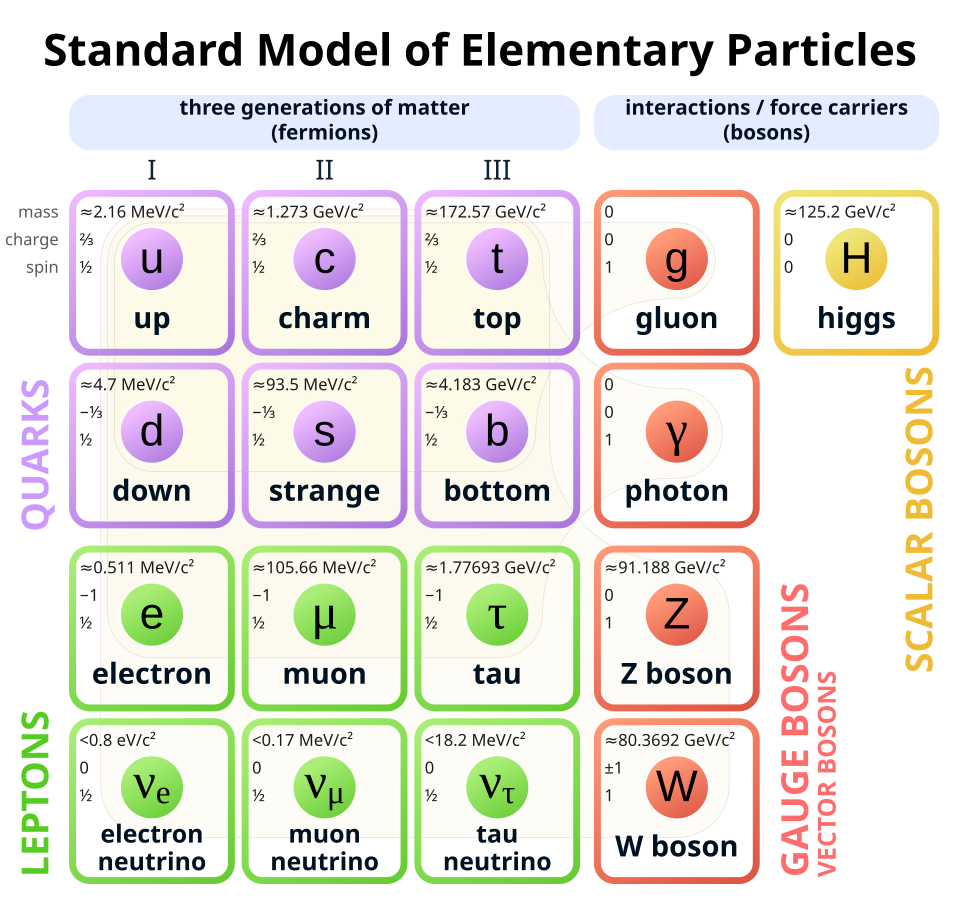
\includegraphics[width=0.85\linewidth, alt={Diagram of the Standard Model elementary particles, organized by quarks, leptons, gauge bosons, and the Higgs boson, with their masses, charges, and spins labeled.}]{figures/ch2/particle_content}
  \caption{The elementary particles of the Standard Model. The dynamics of the 6 quarks and the 8 gluons (all gluon fields are represented by one box in the diagram), described by the theory of quantum chromodynamics, is most relevant to this thesis. Figure reproduced from Ref.~\cite{Cush:SMdiagram} under the CC~3.0 license.}
  \label{fig:sm-particles}
\end{figure}

% Define some colors for grouping
\definecolor{quarkcolor}{rgb}{0.95, 0.88, 0.88}
\definecolor{leptoncolor}{rgb}{0.88, 0.92, 0.95}
\definecolor{bosoncolor}{rgb}{0.92, 0.95, 0.88}
\definecolor{higgscolor}{rgb}{0.95, 0.92, 0.82}
\definecolor{headercolor}{rgb}{0.25, 0.25, 0.35}

\begin{table}[ht]
    \centering
    \caption{Standard Model particles and their representations under the gauge group
    $SU(3)_c \times SU(2)_L \times U(1)_Y$. Representations are written as
    $(\mathbf{d_3},\, \mathbf{d_2},\, Y)$, where $d_3$ and $d_2$ are the
    dimensions of the $SU(3)_c$ and $SU(2)_L$ representations, and $Y$ is the
    weak hypercharge under the convention $Q = T_3 + Y/2$.
    Three generations of fermions are implied; all carry identical quantum numbers.}
    \label{tab:sm-reps}
    \renewcommand{\arraystretch}{1.4}
    \begin{tabular}{%
      >{\raggedright}p{3.6cm}
      >{\centering}p{2.2cm}
      >{\centering}p{3.2cm}
      c
    }
        \toprule
        \rowcolor{headercolor}
        \textcolor{white}{\textbf{Particle}} &
        \textcolor{white}{\textbf{Symbol}} &
        \textcolor{white}{\textbf{Representation}} &
        \textcolor{white}{\textbf{Spin}} \\
        \midrule
        
        \multicolumn{4}{l}{\textit{\textbf{Quarks (Left-handed doublets)}}} \\[2pt]
        \rowcolor{quarkcolor}
        Quark doublet & $Q_L = \binom{u}{d}_{\!L}$ & $(\mathbf{3},\,\mathbf{2},\,+\tfrac{1}{3})$ & $1/2$ \\
        
        \midrule
        \multicolumn{4}{l}{\textit{\textbf{Quarks (Right-handed singlets)}}} \\[2pt]
        \rowcolor{quarkcolor}
        Up-type quark & $u_R$ & $(\mathbf{3},\,\mathbf{1},\,+\tfrac{4}{3})$ & $1/2$ \\
        \rowcolor{quarkcolor}
        Down-type quark & $d_R$ & $(\mathbf{3},\,\mathbf{1},\,-\tfrac{2}{3})$ & $1/2$ \\
        
        \midrule
        \multicolumn{4}{l}{\textit{\textbf{Leptons (Left-handed doublets)}}} \\[2pt]
        \rowcolor{leptoncolor}
        Lepton doublet & $L_L = \binom{\nu_e}{e}_{\!L}$ & $(\mathbf{1},\,\mathbf{2},\,-1)$ & $1/2$ \\
        
        \midrule
        \multicolumn{4}{l}{\textit{\textbf{Leptons (Right-handed singlets)}}} \\[2pt]
        \rowcolor{leptoncolor}
        Charged lepton & $e_R$ & $(\mathbf{1},\,\mathbf{1},\,-2)$ & $1/2$ \\
        
        \midrule
        \multicolumn{4}{l}{\textit{\textbf{Gauge Bosons}}} \\[2pt]
        \rowcolor{bosoncolor}
        Gluons & $g^a_\mu$ & $(\mathbf{8},\,\mathbf{1},\,0)$ & $1$ \\
        \rowcolor{bosoncolor}
        $W$ bosons & $W^i_\mu$ & $(\mathbf{1},\,\mathbf{3},\,0)$ & $1$ \\
        \rowcolor{bosoncolor}
        $B$ boson & $B_\mu$ & $(\mathbf{1},\,\mathbf{1},\,0)$ & $1$ \\
        
        \midrule
        \multicolumn{4}{l}{\textit{\textbf{Higgs Sector}}} \\[2pt]
        \rowcolor{higgscolor}
        Higgs doublet & $H$ & $(\mathbf{1},\,\mathbf{2},\,+1)$ & $0$ \\
        
        \bottomrule
    \end{tabular}
\end{table}


This chapter provides a very high level overview of quantum chromodynamics (QCD), with a focus on the aspects of the theory relevant to the Large Hadron Collider (LHC).
It does not survey the Standard Model or QCD with any completeness.
Instead the goal is to motivate two of the observables measured in Chapter~\ref{ch:zjets} from first principles.
They will be introduced in Sections~\ref{sec:eec} and~\ref{sec:id}.

QCD is our current best theory of the strong nuclear force.
It affects the dynamics of all particles that carry color charge, meaning they transform under a non-trivial representation of the $\mathrm{SU}(3)_c$ sub-group of the Standard Model gauge group:
\begin{equation}
  \mathrm{SU}(3)_c \times \mathrm{SU}(2)_L \times \mathrm{U}(1)_Y
  \label{eqn:sm_gauge_group}
\end{equation}
The particles of the Standard Model are shown in Figure~\ref{fig:sm-particles}.
The representations of each of the fundamental fields of the Standard Model (grouped as quarks, leptons, gauge bosons, and the Higgs doublet fields) are shown in Table~\ref{tab:sm-reps}.
All of the fundamental fields transform in the singlet representation of $\mathrm{SU}(3)_c$ except for the quarks and gluons.
These are the particles that carry color charge and participate in strong-force dynamics.
The quarks are the massive particles that make up all of the baryonic matter in the universe, and the gluons are the massless gauge bosons that mediate the strong force.
These particles are also the input particles to all LHC collisions.
The LHC is a hadron collider, meaning it collides color neutral bound states of quarks and gluons.
The measurement in Chapter~\ref{ch:zjets} is of a cross section measured in proton--proton collisions at $\sqrt{s} = 13$~TeV.
Almost all of the LHC collisions recorded by the ATLAS detector contain strong dynamics, making grappling with the complexities of this force a central challenge of LHC physics.
\textit{Jets} are the experimental signature of the production of high transverse momentum (\pt) color-charged particles.
Jets will be introduced in Section~\ref{sec:jets}, and two methods for studying them will be introduced in Sections~\ref{sec:eec} and~\ref{sec:id}.

\section{Jets and Jet Substructure at the LHC}
\label{sec:jets}

\subsection{The QCD Lagrangian and Asymptotic Freedom}

QCD dynamics are set by the Lagrangian,
\begin{equation}
  \mathcal{L}_{\mathrm{QCD}} = -\frac{1}{4} G^a_{\mu\nu} G^{\mu\nu}_a + \sum_f \bar{q}_f \left( i \gamma^\mu D_\mu - m_f \right) q_f,
  \label{eqn:qcd_lagrangian}
\end{equation}
where $G^a_{\mu\nu}$ is the gluon field strength tensor, the sum runs over the six quark flavors $f$, $D_\mu = \partial_\mu - i g_s T^a A^a_\mu$ is the covariant derivative, $g_s$ is the strong coupling constant, and $T^a$ are the generators of $\mathrm{SU}(3)$.
The gluon field strength tensor is
\begin{equation}
  G^a_{\mu\nu} = \partial_\mu A^a_\nu - \partial_\nu A^a_\mu + g_s f^{abc} A^b_\mu A^c_\nu,
  \label{eqn:field_strength}
\end{equation}
where $f^{abc}$ are the $\mathrm{SU}(3)$ structure constants and $A^a_\mu$ are the gluon fields.

A critical difference between QCD and QED is that the structure constants $f^{abc}$ in Equation~\ref{eqn:field_strength} are non-zero for the $\mathrm{SU}(3)$ gauge group of QCD.
The presence of non-zero structure constants introduces cubic and quartic gluon self-interaction vertices in the Feynman rules, allowing the eight gluon fields to couple to each other, as shown in Figure~\ref{fig:gluon-vertices}.
The result is that each gluon field itself carries color charge.
In QED, no analogous photon self-coupling exists and the photon does not carry electric charge.

\begin{figure}[ht]
  \centering
  \begin{subfigure}[b]{0.45\textwidth}
    \centering
    \begin{tikzpicture}
      \begin{feynman}
        \vertex [particle=\(g\)] (g1) at (-1.3, 0.9);
        \vertex [particle=\(g\)] (g2) at (-1.3, -0.9);
        \vertex (v1) at (0, 0);
        \vertex [particle=\(g\)] (g3) at (1.3, 0);
        \diagram* {
          (g1) -- [gluon] (v1) -- [gluon] (g3),
          (g2) -- [gluon] (v1),
        };
      \end{feynman}
    \end{tikzpicture}
    \caption{Three-gluon vertex ($\sim g_s f^{abc}$)}
    \label{fig:3g-vertex}
  \end{subfigure}
  \hfill
  \begin{subfigure}[b]{0.45\textwidth}
    \centering
    \begin{tikzpicture}
      \begin{feynman}
        \vertex [particle=\(g\)] (g1) at (-1.3, 0.9);
        \vertex [particle=\(g\)] (g2) at (-1.3, -0.9);
        \vertex (v) at (0, 0);
        \vertex [particle=\(g\)] (g3) at (1.3, 0.9);
        \vertex [particle=\(g\)] (g4) at (1.3, -0.9);
        \diagram* {
          (g1) -- [gluon] (v) -- [gluon] (g3),
          (g2) -- [gluon] (v) -- [gluon] (g4),
        };
      \end{feynman}
    \end{tikzpicture}
    \caption{Four-gluon vertex ($\sim g_s^2 f^{abe} f^{cde}$)}
    \label{fig:4g-vertex}
  \end{subfigure}
  \caption{The gluon self-interaction vertices that arise from the non-Abelian structure of QCD.}
  \label{fig:gluon-vertices}
\end{figure}

These self-coupling diagrams have important consequences for the running of the strong coupling constant $g_s$.
For the electromagnetic interactions, the coefficient of the one-loop beta function is positive, meaning the coupling increases with the energy scale.
For the strong interactions, the gluon self-interaction contributes a large negative term to the one-loop beta function,
\begin{equation}
  \mu \frac{dg_s}{d\mu} = -\frac{g_s^3}{16\pi^2} \left( \frac{11}{3} C_A - \frac{4}{3} T_F n_f \right) + \mathcal{O}(g_s^4),
  \label{eqn:beta_function}
\end{equation}
where $C_A = 3$ is the adjoint Casimir, $T_F = 1/2$, and $n_f$ is the number of active quark flavors.
The first term in the parentheses is the important one that arises from the gluon-gluon self interaction.
For $n_f \leq 16$ the quantity in the parentheses is positive, making the overall sign negative, so $g_s$ decreases as the energy scale $\mu$ increases.
This is in contrast to the electromagnetic interactions whose strength increases with energy scale.
The running of the QCD coupling constant, verified by many experimental measurements, is illustrated in Figure~\ref{fig:qcd_running}.
\begin{figure}[ht]
  \centering
  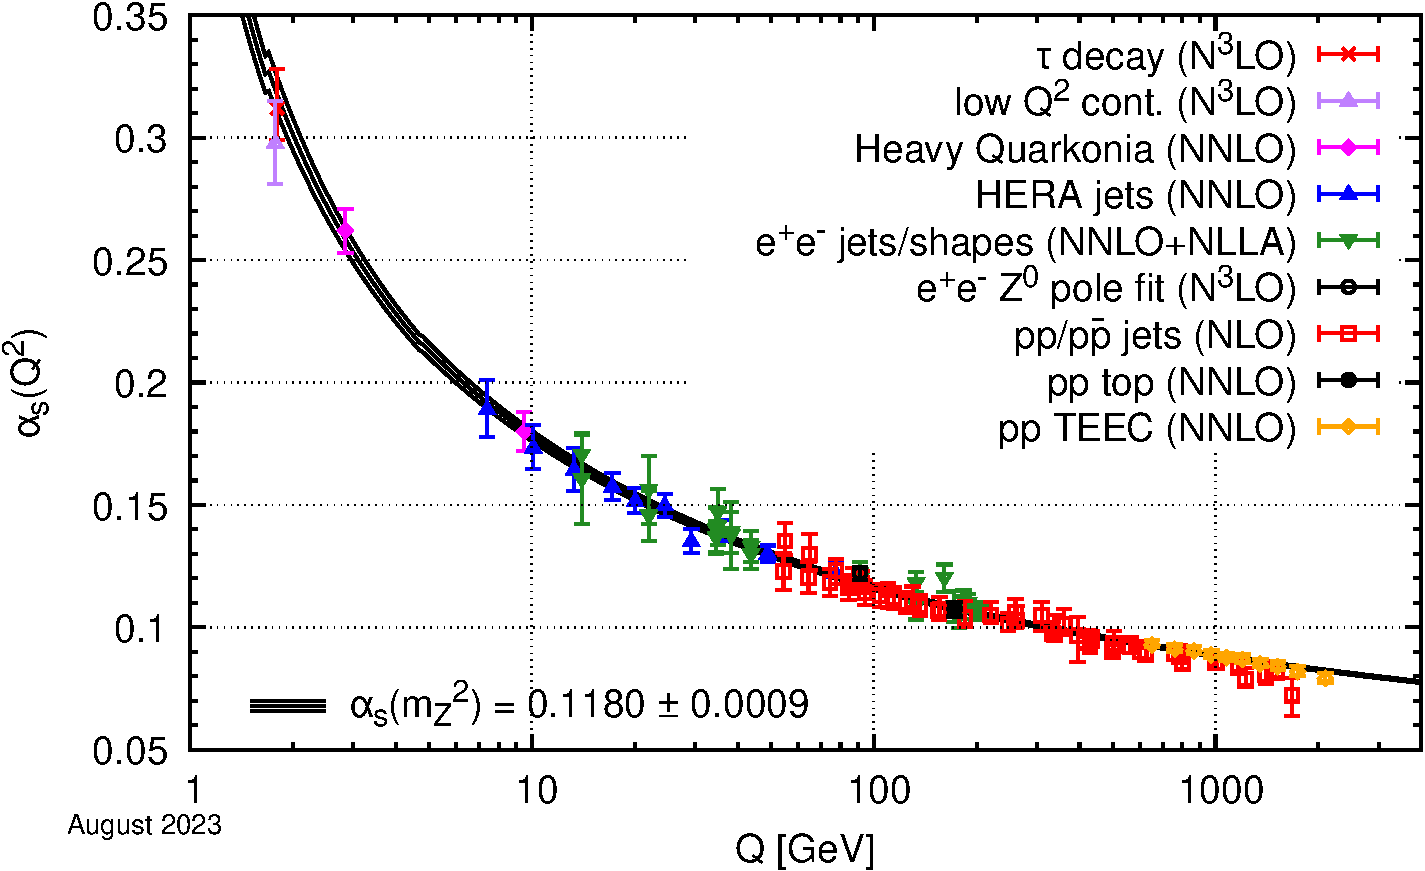
\includegraphics[width=0.75\linewidth, alt={Compilation plot of measurements of the strong coupling alpha sub s as a function of the energy scale Q, showing that the coupling decreases as Q increases over a wide range of energies.}]{figures/ch2/alphas-v-Q-2023-cropped.pdf}
  \caption{A compilation of experimental measurements of the strong coupling $\alpha_s$ as a function of the energy scale $Q$, illustrating asymptotic freedom through the decrease of the coupling at high energies. Figure reproduced from Ref.~\cite{Huston:2023ofk} under a CC~BY~4.0 license.}
  \label{fig:qcd_running}
\end{figure}
At high energy scales $Q$, the strong coupling (here plotting $\alpha_s$ rather than $g_s$) is less than 0.1.
This is the perturbative QCD regime in which a perturbative expansion in powers of the strong coupling is well defined.
Here the strong force dynamics are similar to the EM dynamics and color charged particles can freely propagate.
At low energy scales the coupling begins to diverge.
Below the QCD hadronization scale $\Lambda_{\mathrm{QCD}} \sim 200$~MeV, the strong force is so powerful that it becomes energetically favorable for color-charged particles to pull opposite color-charged particles out of the vacuum such that the overall color charge is neutralized.
This is known as \textit{hadronization}, since color charged particles like quarks and gluons become bound up in composite particles known as hadrons.
The protons and neutrons inside atomic nuclei are the most important hadrons, as they make up the vast majority of the baryonic matter in the universe.
Hadronization is an inherently non-perturbative process since the strong coupling constant is large by assumption.
The decreasing strength of the strong force with energy scale is known as asymptotic freedom\cite{Gross:1973id, Politzer:1973fx}.
It offers an example of how an energy scale (namely $\Lambda_{\mathrm{QCD}}$) can be generated by the structure of a theory rather than being set by free parameters as is the case for many of the theoretical issues described in Chapter~\ref{ch:intro}.

\subsection{Parton Showers}

At high energies, quarks and gluons can propagate freely but this does not mean that the propagation is simple.
The QCD splitting functions, which describe the probability of a parton\footnote{Quarks and gluons are often referred to as partons, since they are the constituent parts of the hadrons we observe at low energies. At high energies, the term is still used but is less descriptive since quarks and gluons can propagate freely.} to emit a gluon, have soft and collinear divergences.
The leading-order splitting function is given schematically by
\begin{equation}
  dP = \frac{\alpha_s}{\pi} C_f \frac{d\epsilon}{\epsilon}\frac{d\theta^2}{\theta^2}
  \label{eqn:splitting}
\end{equation}
where $\epsilon = 1 - z$ is one minus the momentum fraction carried by one of the daughter partons $z$, $C_F = 4/3$ is the fundamental Casimir of $\mathrm{SU}(3)$, and $\theta$ is the emission angle between the daughter partons.
This splitting function diverges as either $\epsilon$ or $\theta$ become small, corresponding to the emission of a soft or collinear gluon by the parent parton.
These divergences exist whether the parent parton is a quark or a gluon, so gluons emitted by an initiating parton can in-turn emit more gluons.
This cascade of largely soft and collinear gluons is known as a \textit{parton shower}, which continues until all of the emitted partons reach energies near $\Lambda_{\mathrm{QCD}}$.

Any quark or gluon produced in an LHC collision immediately undergoes a parton shower before it can interact with a detector.
Given the collinear divergence of the splitting function the shower is collimated, meaning all of the resulting quarks and gluons travel roughly in the same direction.

\subsection{Jets}

These two processes, parton showering at high energies and hadronization at low energies, imply that the result of the production of a high \pt quark or gluon in an LHC collision is a collimated spray of hadrons that can interact with a detector.
This signature is known as a \textit{jet}.
Measurement of a jet requires that the four-vectors of hadrons within a jet, typically called \textit{jet constituents}, be measured by the detector.
The four-vector of the jet itself can be calculated by summing the four-vectors of the jet constituents, and then the four-vector of the jet can be used as a stand-in for the four-vector of the initiating parton when analyzing LHC collisions.
This simple prescription has several complications:

\begin{enumerate}
  \item{
    Choosing which hadrons to include in a jet is non-trivial.
    In proton-proton collisions, the presence of multiple jets, multiple parton interactions, and initial and final state radiation significantly complicate this question.
    Studying jets typically requires specifying a \textit{jet clustering algorithm}, which leads to many experimental and theoretical subtleties.
  }
  \item{
    The general purpose detectors on the LHC, ATLAS and CMS, are not sensitive to the entire four-vector for an arbitrary hadron.
    In particular the masses of individual hadrons are not constrained (see \Cref{sec:zjets-uncert-unfold}).
    Significant approximations on hadron masses are made so that the four-vector of the jet can be calculated.
  }
  \item{
    Even the parts of the hadron four-vectors that are measured are not measured with perfect resolution.
    Some smearing of the true kinematic quantities is inevitable, and can cause significant distortions in the four-vector of the jet.
  }
  \item{
    The LHC operates with many proton-proton collisions per bunch crossing.
    The presence of these \textit{pileup collisions} superimposed on top of the collision of interest can contaminate the jet, adding hadrons to it that were not produced by the shower initiated by the parton.
  }
\end{enumerate}

Each of these points adds significant complications to the experimental study of jets, even if the only goal is to infer the four-vector of the initiating parton.
However there is a huge amount of interesting and unknown physics contained in the parton shower and hadronization.
This physics can be probed through examining the underlying measurements of the jet constituents.
Studying this \textit{jet substructure} requires processing the full, high-dimensional data type that describes all hadrons within a jet.
The complexity and high dimensionality of these data types makes them natural applications for deep learning methods.
This is why the jet substructure community saw the earliest and most enthusiastic adoption of deep learning in LHC physics \cite{Larkoski:2017jix, Kogler:2018hem}.

The study of jet substructure is organized around substructure observables.
These are quantities that can be calculated using the four-vectors of the jet constituents that capture certain features of a jet.
As is the case for all physics, the study of jet substructure moves forward through an interplay between theorists and experimentalists.
Theorists make predictions of jet substructure observables within the framework of QCD, and experimentalists make measurements of these observables that can be compared to and used to refine the theory.

There are two approaches to calculating jet substructure observables within QCD.
The first approach is to directly calculate a given observable within perturbative QCD.
A complete calculation involves three ingredients~\cite{Larkoski:2017jix}: (1) a perturbative calculation at some fixed order in $\alpha_s$, (2) resummation of the large logarithms that result from the infrared and collinear divergences described above, and (3) some accounting for non-perturbative effects like hadronization, typically through an analytic shape function.
The result is prediction of the cross section of some process, typically di-jet production in electron--positron or proton--proton collisions, differential in the substructure observable~\cite{Dasgupta:2001sh}.

The second approach is to recursively apply the splitting function in Equation~\ref{eqn:splitting}.
Given the probability of a splitting at a given scale does not depend on splittings at any previous scales, the chain of splittings can be described as a Markov chain, and samples from the probability distribution over the final configuration of the parton shower can be obtained by Markov Chain Monte Carlo (MCMC) methods.
Samples provided by the MCMC are a fully exclusive partonic final state: a list of partons at or above the QCD hadronization scale $\Lambda_{\mathrm{QCD}}$.
In order to compare to experimental measurements, phenomenological models of hadronization can be applied~\cite{Marchesini:1991ch, Sjostrand:2014zea}.
Unlike the parton shower sampling, these models are not based on first principles QCD but are models with free parameters that must be \textit{tuned} to match experimental data.
The combination of fixed-order perturbative calculations, followed by sampling of parton shower configurations through MCMC, followed by application of a hadronization model, produces an \textit{event generator}.
These event generators are capable of simulating proton-proton collisions with high accuracy~\cite{Bierlich:2022pfr,Bellm:2015jjp,Sherpa:2019gpd}.
This approach is very general-purpose, since it can provide predictions for any observable, including those that are too complicated for the analytic approach described above, or even IRC unsafe observables for which the resummation in step 2 above is not possible.
The limitation is that the accuracy of the event generator for a given observable is hard to characterize systematically, so the assigned theory uncertainties are typically less rigorous than those from resummed calculations.

An important practical distinction between these two approaches is how their outputs are presented.
Resummed calculations provide smooth analytic predictions for differential cross sections, while event generators produce discrete lists of final state hadron four-momenta.
Importantly each of these final state hadrons can be passed through a detector simulation, which simulates how the hadron interacts with a particle detector and ultimately generates experimental data~\cite{GEANT4:2002zbu, ATLAS:2010arf}.
Chaining together a fixed order calculation (either in QCD or the SM more generally), parton shower, hadronization model, and detector simulation defines a \textit{simulation chain} capable of producing simulated collision events that resemble the data collected by the experiments at the LHC.
This ability explains why event generators are used copiously in essentially every analysis of LHC data, while resummed calculations are mostly relevant within the sub-field of jet substructure and QCD.
The difference in the format of the results between the two approaches is a subtle but important motivation for the unfolding methods discussed in Chapter~\ref{ch:unfolding}.

The remainder of this chapter discusses two particular jet substructure observables which are measured in \Cref{ch:zjets}: energy correlators and the intrinsic dimensionality of jets.
The reason for exploring these observables in particular is that they are very difficult to unfold with conventional binned methods.
Detailed discussion of this will be delayed until \Cref{ch:zjets}, but some introduction to the observables from a theoretical standpoint is due first.

\section{Energy correlator observables}
\label{sec:eec}

\subsection{Context}

The $N$-point energy correlator (E$N$C) is defined as the energy-weighted $N$-point correlation function of the radiation pattern produced by a particle collision.
This mathematical object is also used in cosmology to study the CMB and in condensed matter physics to study phase transitions and criticality.
See Refs. \cite{Hofman:2008ar, Kologlu:2019mfz} for a formal treatment of these observables that make these connections explicit.
The simplest energy correlator is the two-point energy correlator (E2C or EEC).
Measuring this quantity involves building a histogram of the opening angle between objects produced by a collision, with the histogram entries weighted by the product of the energies of the two objects.
The energy weighting ensures that the observables are infrared and collinear (IRC) safe.
Either individual particles or clustered jets can be used as the input objects \cite{ATLAS:2015yaa, ATLAS:2017qir, ATLAS:2023tgo, CMS:2024mlf}.
Most studies have focused on the properties of the EEC, but higher order correlators are also of some theoretical interest.
For calculating the E$N$C, the number of $N$-tuples of objects grows combinatorially with the particle multiplicity, which makes the measurement substantially more computationally demanding~\cite{Alipour-fard:2024szj}.

The EEC was first used in particle physics as an event-shape observable in the context of electron-positron collisions \cite{Basham:1977iq, Basham:1978bw, OPAL:1991uui, SLD:1994idb} for the extraction of the strong coupling constant $\alpha_s$.
Several of the measurements shown in green in Figure~\ref{fig:qcd_running} are derived from energy correlator measurements in $e^+e^-$ collisions.
These measurements calculated the correlators between hadronic jets, rather than individual particles, so they are best understood as event shape measurements rather the jet substructure measurements. 

\subsection{Energy Correlators as Jet Substructure Observables}

\begin{figure}[ht]
  \centering
  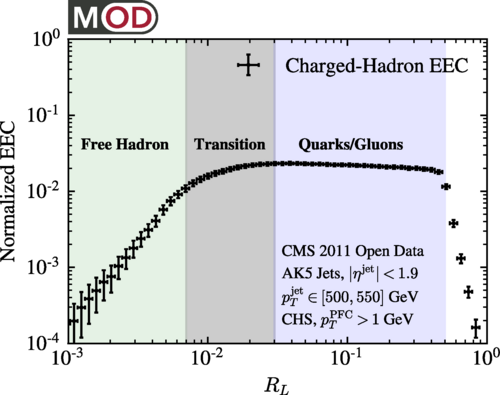
\includegraphics[width=0.65\linewidth, alt={Log-log plot of the normalized two-point energy correlator versus angular scale R sub L for CMS 2011 open data AK5 jets. The figure highlights three regions labeled Free Hadron at low R sub L, Transition at intermediate R sub L, and Quarks/Gluons at larger R sub L.}]{figures/ch2/anec_cms_open.png}
  \caption{The two-point energy correlator (EEC) plotted using CMS open data for high \pt jets, showing distinct free-hadron, transition, and quark/gluon regimes as a function of the angular scale $R_L$ (called $z$ in the text). Figure adapted from Ref.~\cite{Komiske:2022enw} under a CC~BY~4.0 license.}
  \label{fig:cms-open-eec}
\end{figure}

Energy correlators have only recently been used as jet substructure observables.
See Ref.~\cite{Moult:2025nhu} for a recent review.
Interest has been driven by a few properties of the two-point correlator in the highly collinear limit, which is dominated by the highly collimated radiation within jets.
The two-point correlator is given as
\begin{equation}
  EEC(z) = \frac{1}{\sigma} \sum_{i,j} \int d\sigma \frac{E_i E_j}{Q^2} \delta(z - \frac{1- \cos \theta_{ij}}{2})
  \label{eqn:eec}
\end{equation}
where $\sigma$ is the total cross section, $E_i$ is the transverse energy of the $i$-th particle, $Q$ is the sum of the transverse energies of all particles ($\sum_i E_i$), $\theta_{ij}$ is the angle between the three-momentum vectors of the $i$-th and $j$-th particles, and $z = \frac{1- \cos \theta_{ij}}{2}$.
The first property is that in perturbative QCD, the EEC is predicted to scale as a power law as a function of the opening angle $z$ between freely propagating partons.
The exponent of this power law is related to a formal field theoretical quantity known as the cusp anomalous dimension.
This provides a direct connection between a measurable observable and a fundamental property of QCD.
The larger the angular separation between particles $z$, the earlier in the jet formation process (or the higher the energy) is being probed, since larger angular separations are produced by earlier splittings in the parton shower.
This means that at moderate values of $z$, where particles are contained within a jet but last interacted with each other early in the jet formation process, a power law scaling in the EEC should be observed.

Second, deviations from this perturbative power-law scaling encode non-perturbative effects like hadronization.
As $z$ grows smaller, the EEC quantifies correlations between increasingly collinear particles, meaning they were emitted later in the jet formation process.
Therefore the very small $z$ regime should be sensitive to dynamics below the scale $\Lambda_{\mathrm{QCD}}$ where hadronization occurs.
Hadrons are color neutral and do not interact by the strong force, and so the correlation should reflect non-interacting particles.
Namely it should have a linear dependance on the angular separation.

The combination of these two properties mean that two distinct scaling regimes should be visible in the EEC: a power law corresponding to freely propagating partons at high energies at high $z$, and a linear scaling corresponding to non-interacting hadrons at low $z$.
Ref.~\cite{Komiske:2022enw} first illustrated these two distinct scaling regimes using CMS open data, as shown in \cref{fig:cms-open-eec}.
The two scaling regimes are shaded in blue and green respectively, with a transition regime corresponding to the hadronization process linking them.
The scaling regimes are very well understood from a theoretical standpoint, but the transition between them is intractable given our current theoretical tools, motivating it as a useful regime to measure experimentally.
Measuring the transition requires jets with a high energy (or \pt at a hadron collider) so that a sizeable portion of the parton shower evoluation occurs the hadronization scale.
At LEP, the available center-of-mass energy limited the maximum jet energy to around 100~GeV, which is too low to observe the perturbative scaling regime cleanly and helps explains why energy correlators were relatively unexplored as jet substructure tools in the $e^+e^-$ era.
However the large center-of-mass energies of the LHC produce the needed high \pt jets in large numbers.

The final property is that the energy correlators can be calculated to very high perturbative accuracy.
The EEC in $e^+e^-$ collisions has been computed to next-to-next-to-next-to-leading order (N$^3$LO), which is a very high level of accuracy for a jet substructure quantity~\cite{Ebert:2020sfi}.
Recent work has provided N$^3$LL accurate predictions for energy correlator observables in proton--proton collisions as well~\cite{Gao:2023ivm}.

\subsection{Experimental Status}

The renewed interest in energy correlator observables from the theory community has produced many new measurements of the observables.
I only summarize here energy correlator measurements using particles, rather than jets, since this is needed to access the collinear regime.

The most relevant existing measurement is of the EEC and E3C observables by the CMS collaboration in proton-proton collisions at the LHC.
This paper also used the measured spectra to extract $\alpha_s$~\cite{CMS:2024mlf}.
This is the only published measurement using high \pt jets from $pp$ collisions at the LHC, so it serves as a useful comparison for the EEC measurement in \Cref{sec:zjets-results-eec}.
The ALICE collaboration additionally measured the EEC in charm-tagged jets in proton-proton collisions, but at a lower center-of-mass energy and with less luminosity~\cite{ALICE:2025igw}.
Energy correlator measurements have also been carried out in heavy-ion~\cite{ALICE:2024dfl, CMS:2025ydi} and proton-ion~\cite{Liang-Gilman:2025gjl} collisions at the LHC.
These measurements feature lower \pt jets, where the observed EEC distributions are modified due to interaction with the quark-gluon plasma.
The STAR collaboration has measured the EEC in proton--proton collisions at the lower center of mass energies available at RHIC \cite{STAR:2025jut}.
Legacy analyses have reprocessed archived data from the ALEPH experiment at LEP \cite{Bossi:2024qeu}, where the EEC is measured with all tracks given the substantially lower particle multiplicity produced by electron-positron collisions.
Finally, the H1 collaboration has presented preliminary results measuring the EEC distribution in electron-proton deep inelastic scattering events using all tracks~\cite{H1:prelim}.
This result is particularly relevant because it uses the same approach to unfolding as the measurement in this thesis.
It will be discussed in detail in Chapter~\ref{ch:unfolding}.
\Cref{tab:eec-measurements} summarizes the experimental landscape.

\begin{table}[t]
    \caption[Summary of published experimental measurements of energy-energy correlator observables.]{
      Summary of published experimental measurements of energy-energy correlator observables using particles.
      Jet transverse-momentum ranges are approximate and refer to the leading-jet or inclusive-jet selection;
      a dash (--) indicates measurements performed on all final-state particles without jet clustering.
      The asterisk denotes measurements made with charged-particle jets rather than jets that include the neutral component.
      The dagger denotes preliminary results.}
    \label{tab:eec-measurements}
    \centering
    \small
    \NoHyper
    \begin{tabularx}{\linewidth}{
      >{\centering\arraybackslash}X
      >{\centering\arraybackslash}X
      >{\centering\arraybackslash}X
      >{\centering\arraybackslash}X
      >{\centering\arraybackslash}X
    }
      \toprule \toprule
      Experiment & System & $\sqrt{s}$ & Observable & Jet $p_T$ range \\
      \midrule
      ALEPH~\cite{Bossi:2024qeu} & $e^+e^-$ & 91.2~GeV  & E2C all tracks    & -- \\
      CMS~\cite{CMS:2024mlf}           & $pp$     & 13~TeV        & E2C, E3C inside jets & 500--2500~GeV \\
      ALICE~\cite{ALICE:2025igw}       & $pp$     & 13~TeV        & E2C inside jets & 10--30~GeV* \\
      ALICE~\cite{ALICE:2024dfl}       & $pp$     & 5.02~TeV      & E2C inside jets & 20--80~GeV* \\
      STAR~\cite{STAR:2025jut}         & $pp$     & 200~GeV       & E2C inside jets & 25--55~GeV \\
      ALICE$^\dagger$~\cite{Liang-Gilman:2025gjl} & $pPb$ & 5.02~TeV & E2C inside jets & 20--80~GeV* \\
      CMS~\cite{CMS:2025ydi}           & $\text{PbPb}$ & 5.02~TeV & E2C inside jets & 120--200~GeV \\
      H1$^\dagger$~\cite{H1:prelim}              & $ep$     & 320~GeV       & E2C all tracks & -- \\
      \bottomrule \bottomrule
    \end{tabularx}
    \endNoHyper
  \end{table}

There are three important gaps in the existing measurements.
First, there is only one measurement from CMS which uses the high \pt jets provided by the LHC to measure the EEC well above the confinement scale~\cite{CMS:2024mlf}.
A similar measurement performed by ATLAS would be a valuable contribution.
Second, all current LHC measurements cluster particles into jets before performing the correlator measurement on the jet substructure.
This is experimentally convenient, especially for the extraction of a universal hadronization scale and for the necessary unfolding procedure discussed in \Cref{ch:unfolding}, but it introduces dependencies on the jet clustering algorithm applied and prevents measurement of the EEC over a full range of angular separations.
A measurement performed on all particles in the event, without prior jet clustering, would allow measurement of the entire perturbative scaling regime without the distribution being cut-off due to the jet radius.
Third, all existing measurements use only charged particles, since neutral particles such as photons and neutral pions are measured with substantially worse angular resolution.
Theoretical predictions for charged-particle-only measurements require the track function formalism~\cite{Chang:2013rca, Chang:2013iba}, which introduces more complexity.
Discussion of this is beyond the scope here, but work on this formalism and associated measurements is on-going~\cite{ATLAS:2025qtv} providing a promising path to calculation of energy correlators on charged particle final states.
One of the primary physics contributions of the measurement presented in this thesis is to address the first two gaps, with the third being left as a fundamental limitation of current detector technology.

\section{Intrinsic Dimensionality of Jets}
\label{sec:id}

The energy-energy correlators discussed in Section~\ref{sec:eec} are jet substructure observables that are of interest because of their connections to the underlying theory of QCD.
In contrast, the intrinsic dimensionality of jets is an observable motivated by a basic question about the structure of the data rather than ties to the underlying theory.
This is a very new observable that has only been treated, to my knowledge, in a few research papers~\cite{Komiske:2019fks, DAgnolo:2025qqr}.
There are likely interesting connections to the underlying theory.
For example the scale dependence of the intrinsic dimension (see below) could in principle encode information about the parton shower branching structure, but this remains an essentially unexplored topic.
Part of the motivation for measuring this observable is to demonstrate that measurements of it are possible, hopefully motivating further theoretical work.
The rest of the motivation is to demonstrate that deep learning methods allow us to ask questions about the data in its native, high dimensionality.

\subsection{The Manifold Hypothesis and Intrinsic Dimensionality}

The manifold hypothesis states that high-dimensional data generated by natural processes tend to cluster on lower-dimensional manifolds embedded in the high-dimensional space.
Put another way, the naive high dimensional representation we use to describe the data is redundant.
Fewer coordinates are needed to describe the data than the naive dimensionality would suggest, demonstrating that there is structure in the high dimensional space that is invisible to humans examining projections (e.g. histograms or scatter plots) but easily identifiable for deep learning models.
This observation is implicitly known in particle physics, given our data is known to be generated by relatively simple processes and respect certain symmetries, but it has not been explicitly quantified.

The intrinsic dimension (ID) of a dataset is the dimension of the underlying manifold.
The manifold hypothesis states that the intrinsic dimension of a dataset is typically much less than the number of naive coordinates we use to describe the data.
An important feature of the ID is that it is \textit{scale-dependent}.
Figure~\ref{fig:id_scale} provides a visual illustration of this scale dependence.
The data cluster on a manifold embedded in the naive three-dimensional coordinates used to describe the data, but the apparent dimension of the manifold depends on the length scale.
At large distances the manifold looks like a curve that can be parametrized with one free parameter, so the dimension is one.
At smaller distances, the noise in the data gets resolved and the manifold appears first two- and then three-dimensional.
Clearly the intrinsic dimension also does not need to be an integer.
Fractal (non-integer) dimensions are expected as interpolations betwen the dimensions illustrated in the Figure.

\begin{figure}[t]
  \centering
  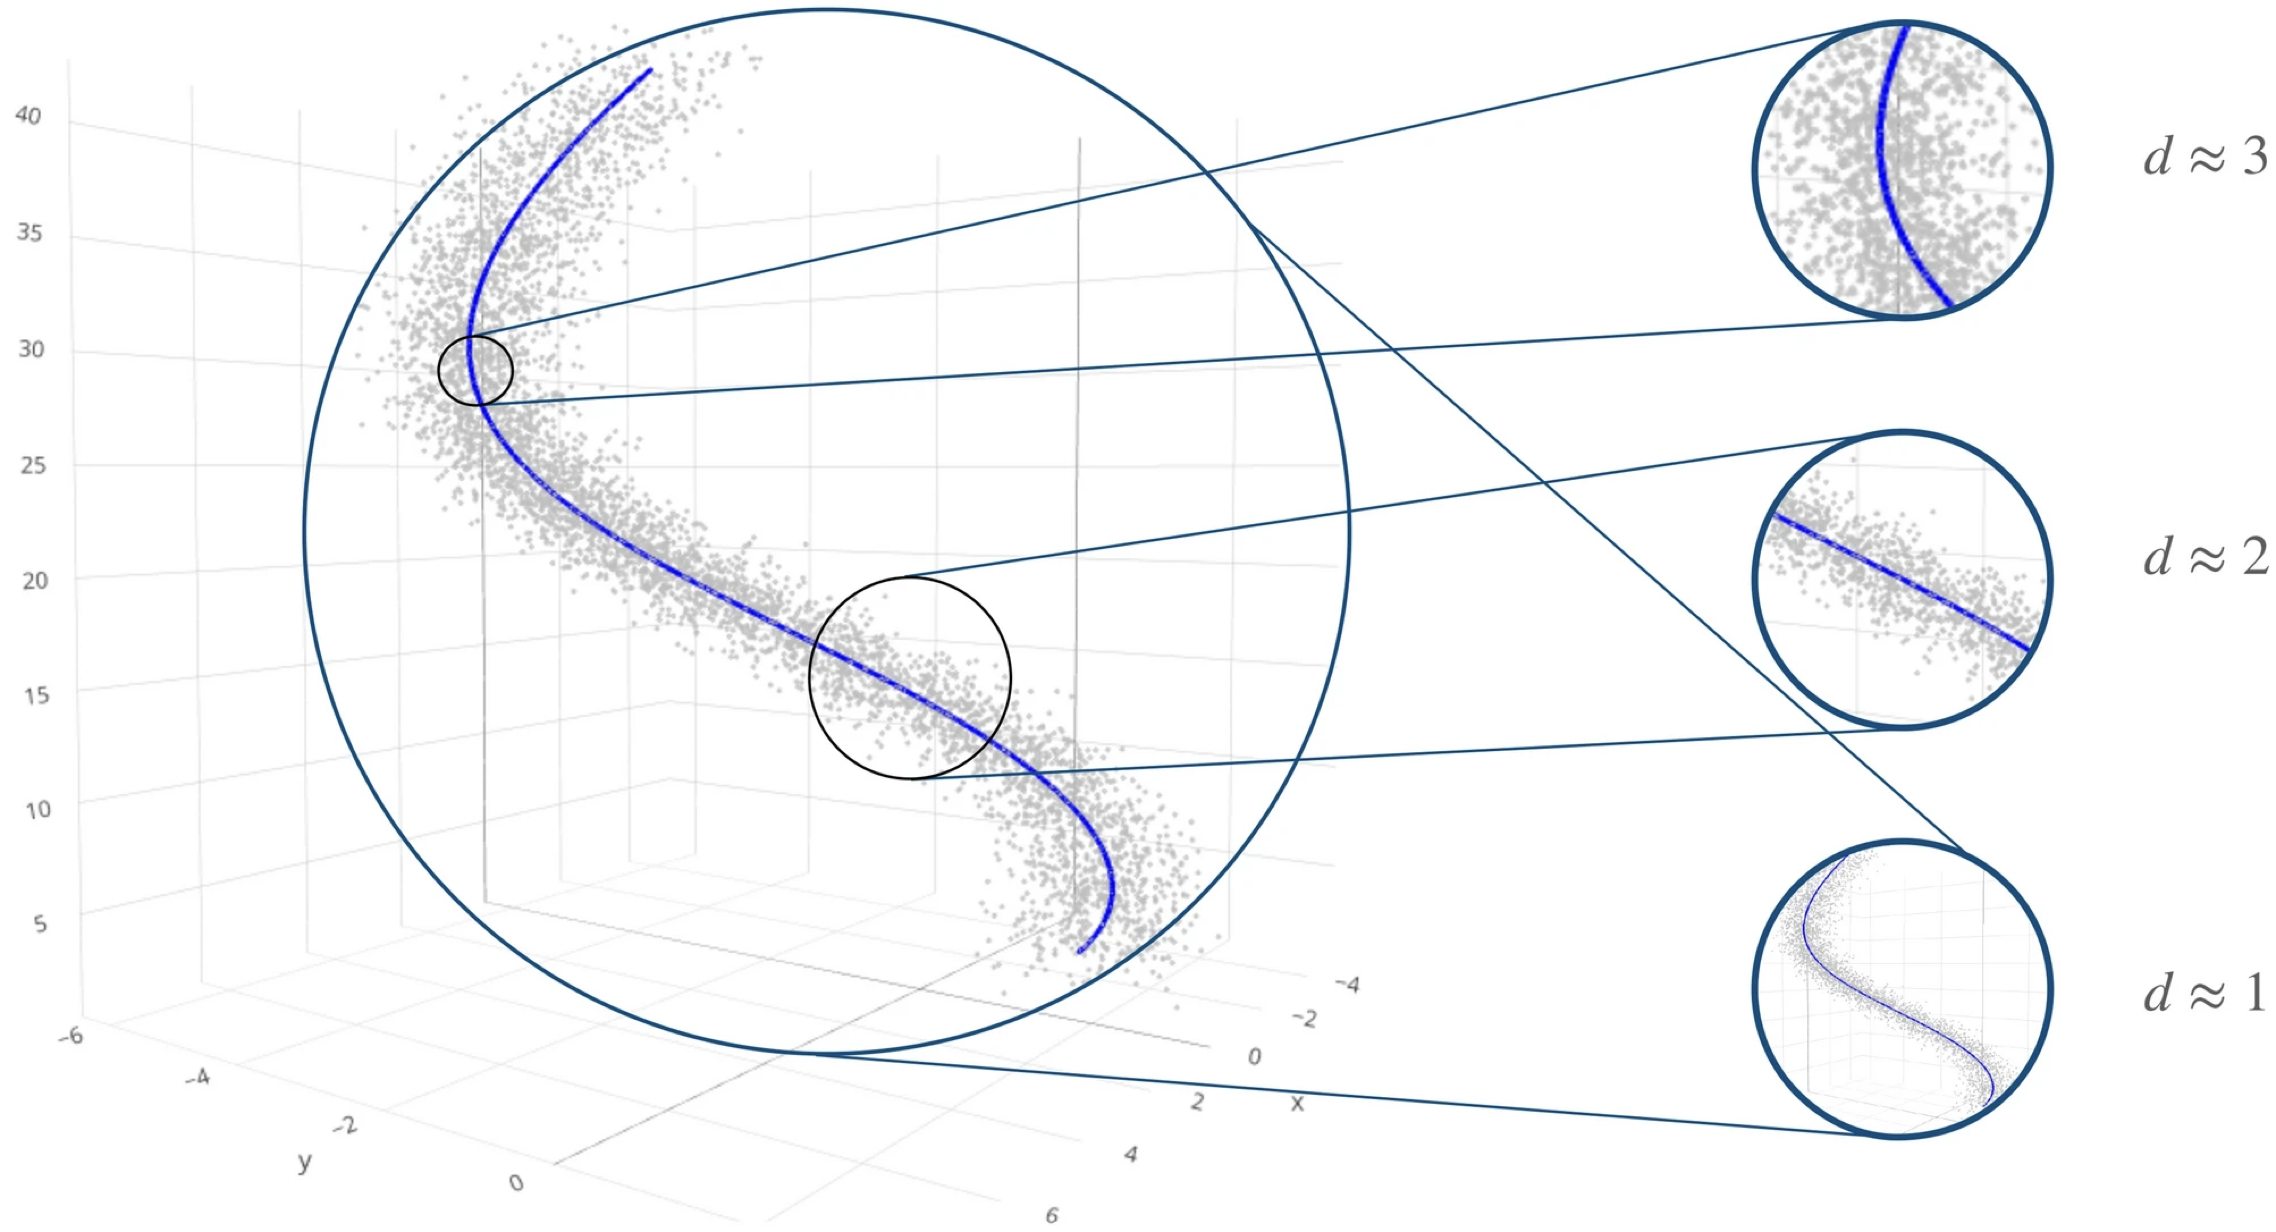
\includegraphics[width=0.85\linewidth, alt={Illustration of the scale dependence of the intrinsic dimension of a dataset, showing that at large distances the data appear zero-dimensional while at smaller scales their manifold structure is revealed.}]{figures/ch2/id_scale}
  \caption{Illustration of the scale dependence of the intrinsic dimension. At large length scales the data appear as a single point (zero dimensions); at smaller scales the geometry of the underlying data manifold becomes visible and the estimated dimension increases. Figure adapted from Ref.~\cite{id-figure} under a CC~BY~4.0 license.}
  \label{fig:id_scale}
\end{figure}

A variety of intrinsic dimension estimators have been proposed~\cite{10.1109/T-C.1971.223208, PhysRevLett.50.346, NIPS2004_74934548, CERUTI20142569, Albergante:2019ijcnn}.
A quick summary is as follows:

\begin{enumerate}
  \item{
    Principal component analysis (PCA) methods count the number of eigenvalues of the data covariance matrix that are statistically distinguishable from zero.
    They assume the data lie on a linear subspace, which is not true of curved manifolds \cite{10.1109/T-C.1971.223208}.
  }
  \item{
    Fractal and correlation dimension methods exploit how the number of data points contained within a ball of radius $r$ as $r$ scales given the dimensionality of a manifold.
    The correlation dimension~\cite{PhysRevLett.50.346} is the most widely used estimator in this family.
    This was also the first estimator to be explored for applications in particle physics~\cite{Komiske:2019fks}.
  }
  \item{
    Maximum likelihood methods write the likelihood of the observed distances between neighboring data points conditioned on the underlying dimensionality~\cite{NIPS2004_74934548}.
    apply a maximum likelihood estimator to the distribution of distances between neighboring data points~\cite{NIPS2004_74934548}.
    This is the most broadly applicable class of estimators.
    One example was recently proposed as a test statistic for searches for physics beyond the Standard Model at the LHC \cite{DAgnolo:2025qqr}, and is measured in \Cref{sec:zjets-results-id}.
  }
  \item{
    Concentration-of-measure methods exploit the fact that vectors pointing from one data point to others cluster in particular directions in high dimensional spaces, rather than being uniformly distributed.
    These methods have not yet been applied to particle physics data~\cite{CERUTI20142569, Albergante:2019ijcnn}.
  }
\end{enumerate}

\subsection{The Energy Mover's Distance}

Most intrinsic dimension estimators require that the vector space used to describe the data be equipped with a metric so that pairwise distances between points can be calculated.
For jet data, Ref.~\cite{Komiske:2019fks} introduced the energy mover's distance (EMD) as a natural choice.
The EMD between two jets $\mathcal{E}$ and $\mathcal{E'}$ is defined as the energy cost of rearranging the substructure of one jet into the substructure of the other,
\begin{equation}
  EMD(\mathcal{E}, \mathcal{E'}) = \min_{f_{ij}} \sum_{i,j} f_{ij} \frac{\theta_{ij}}{R} + | \sum_i E_i - \sum_j E_j |,
\end{equation}
where $f_{ij}$ is the optimal transport plan moving energy from particle $i$ in jet $\mathcal{E}$ to particle $j$ in jet $\mathcal{E'}$, $\theta_{ij}$ is the angle between the three-momentum vectors of the $i$ and $j$ particles, and $R$ is the radius of the jets.
The second term accounts for differences in the overall energy normalization between the jets.
The $f_{ij}$ satisfy the following constraints:
\begin{align}
  f_{ij} \geq 0, \\
  \sum_j f_{ij} \leq E_i, \\
  \sum_i f_{ij} \leq E_j, \\
  \sum_{i,j} f_{ij} = E_{min},
\end{align}
Given the cost function for the EMD is weighted by the particle energies, the EMD is infrared and collinear safe.
To use the EMD as a substructure observable, it is useful to preprocess the jets to remove any irrelevant features, such as the location of the jet in the pseudorapidity-azimuth ($\eta$-$\phi$) plane or its rotation.
The standard approach, used throughout, is to apply a lorentz boost and rotation to the jets such that they are centered in the $\eta$-$\phi$ plane, and then rotate the jets about their axis such that the first principle component of the jet radiation pattern points toward the positive $\phi$ axis.

\subsection{The Nearest-Neighbor Intrinsic Dimension Estimator}

Given a set of $N$ jets with EMDs calculated between all pairs (the number of EMDs to compute is $N^2$), the nearest-neighbor intrinsic dimension (NNID) estimator~\cite{NIPS2004_74934548, DAgnolo:2025qqr} constructs a likelihood from the ratios of distances to successive nearest neighbors.
It is an example of a maximum likelihood method in the taxonomy above.
For a jet $k$, the distance ratio between the $j$th and $i$th nearest neighbors is given as,
\begin{equation}
  \mu_{k,ij} = \frac{\mathrm{EMD}(\mathcal{E}_k, \mathrm{NN}_j(k))}{\mathrm{EMD}(k, \mathrm{NN}_i(k))},
  \label{eqn:mu_ratio}
\end{equation}
where $\mathrm{NN}_i(k)$ denotes the $i$th nearest neighbor of jet $k$ by the EMD metric.
These distance ratios depend on the values of the unphysical indices $i$ and $j$.
In what follows, I follow Ref.~\cite{DAgnolo:2025qqr} and set $j = 2i$ throughout, reducing the number of free parameters to one.
An illustration of these ratios is provided for two dimensional data in Figure~\ref{fig:nnid_illustration}.

In a $d$-dimensional space, the ratios $\mu_{k,ij}$ follow a Pareto distribution whose shape parameter encodes the intrinsic dimensionality $d$.
The intrinsic dimension for a given choice of $i$ and $j=2i$ can then be estimated by minimizing the negative log-likelihood,
\begin{align}
 L &= -\sum_{k=1}^{N} \log f(\mu_{k,ij}; d) \notag \\
 &= -N \log d + (1 + i d)\sum_{k=1}^{N} \log \mu_{k,ij} - (j - i - 1)\sum_{k=1}^{N} \log\left(1 - \mu_{k,ij}^d\right).
 \label{eqn:likelihood}
\end{align}
$f(\mu_{k,ij}; d)$ is the Pareto probability density evaluated at the ratio for jet $k$, which has an analytic form written in the second line.
Numerically minimizing Equation~\ref{eqn:likelihood} over $d$ with all jets $k$ included in the sum yields the estimated intrinsic dimension.

\begin{figure}[t]
  \centering
  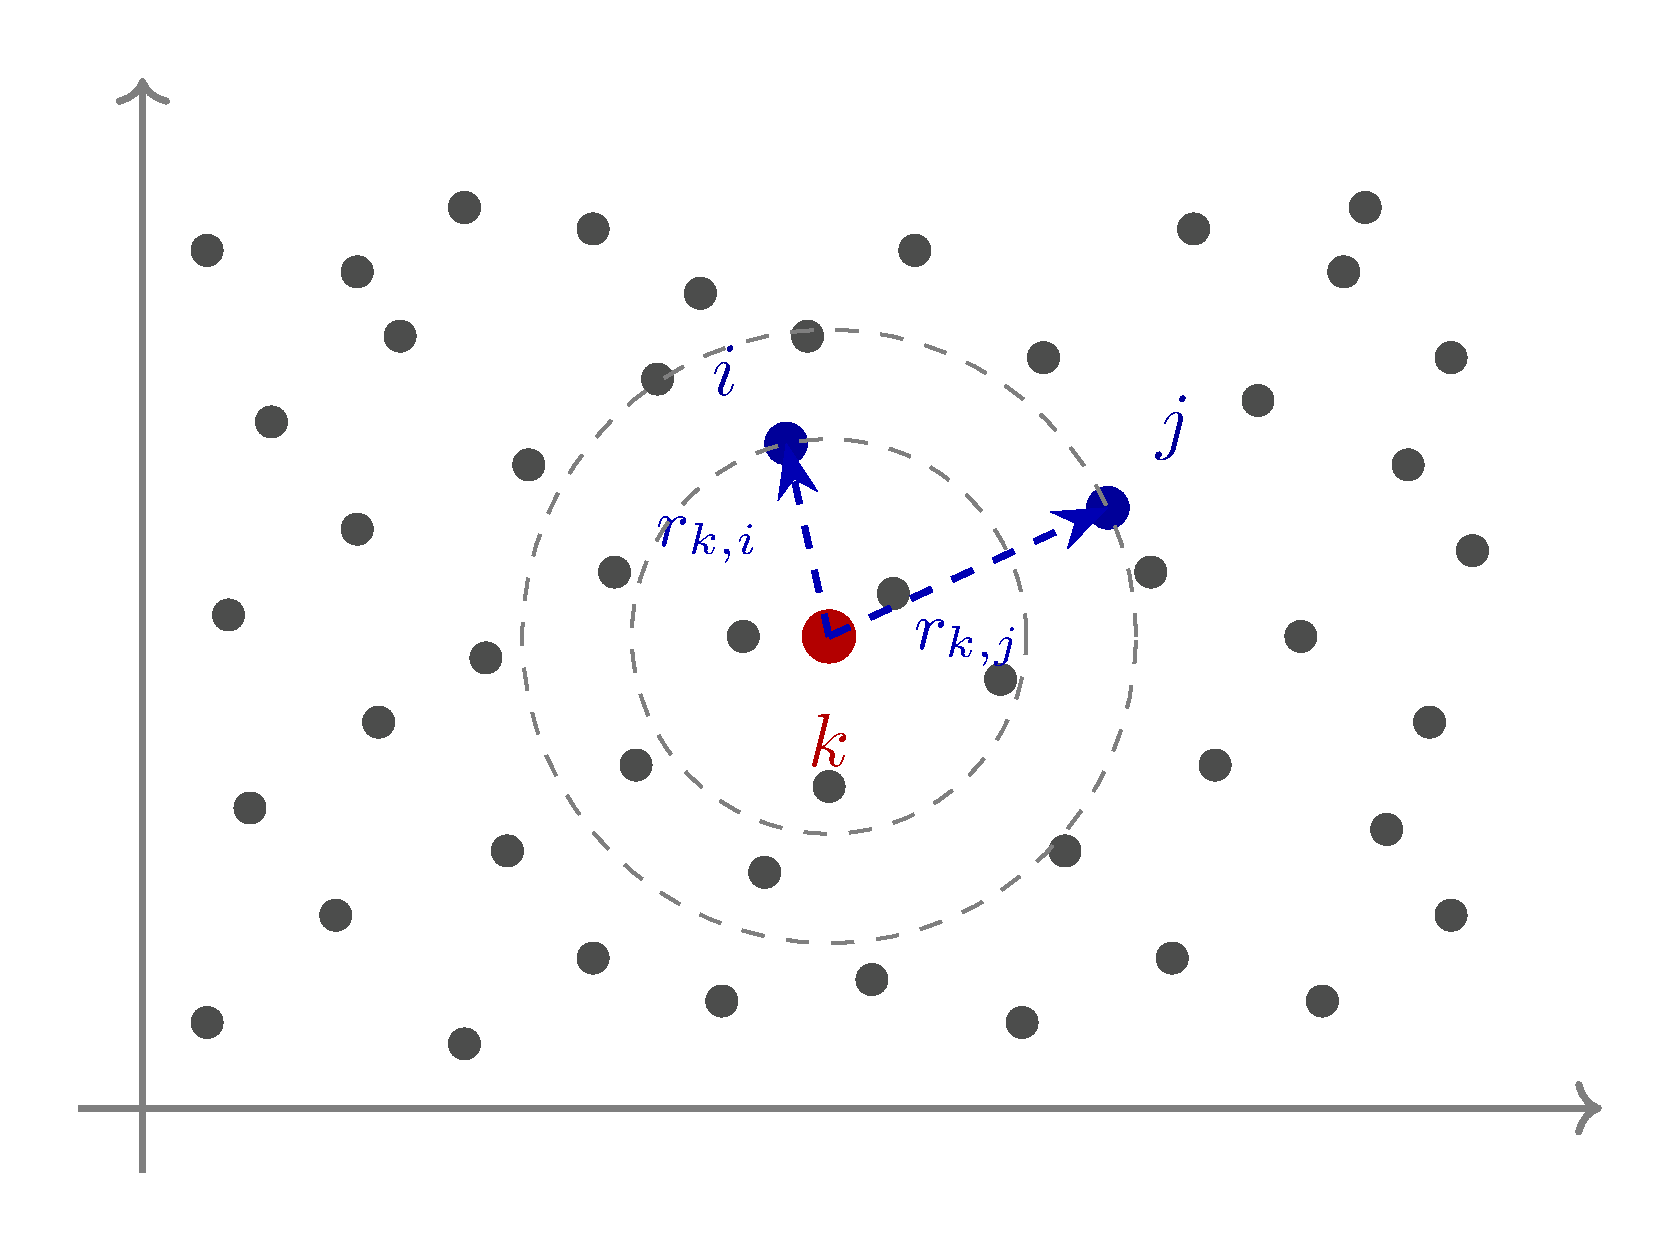
\includegraphics[width=0.7\linewidth, alt={Illustration of the nearest-neighbor intrinsic dimension estimator in a two-dimensional space, showing a reference point and its nearest neighbors at two successive distance scales.}]{figures/ch2/nnid_illustration}
  \caption{Illustration of the NNID estimator in a simple two-dimensional space. For a reference point (center), the distances $r_{k,i}$ to the $i$th nearest neighbor and $r_{k,j}$ to the $j$th nearest neighbor define the ratio $\mu_{k,ij}$. In this particular case $i=5$ and $j=10$. The distribution of these ratios across many reference points encodes the intrinsic dimension of the data manifold.}
  \label{fig:nnid_illustration}
\end{figure}

Each choice of the indices $i$ and $j$ define a new intrinsic dimesionality estimator that will a certain scale in the dataset.
Following fixing $j = 2i$, the choice of $i$ is the only free parameter in the calculation, but this free parameter is unphysical.
It is useful to plot the NNID estimator against a physical scale.
The median EMD between a jet and its $i$th nearest neighbor is a useful, but not unique, choice for this physical scale.
Varying the index $i$ then produces a curve that shows how the NNID estimator evolves with this scale.

Note that particle physics datasets are typically produced with event weights.
This is true for simulated datasets produced by event generators, and for the unbinned spectra that build the cross section measurement in \Cref{ch:zjets}.
The NNID calculation can be extended to accommodate event weights by scaling each jet's contribution to the likelihood in \Cref{eqn:likelihood} by its weight, and replacing the nearest neighbor assignments $i(k)$ and $j(k)$ by their weighted analogues.

\subsection{Generator-Level Results}

Given the novelty of this observable in particle physics, it is worth presenting some generator level results before moving on.
Jets clustered from particle-level charged particles are sampled from the \mgpy and \sherpa samples described in Chapter~\ref{ch:zjets}.
See \Cref{sec:zjets-results-id} for more details.
Each point in the curves corresponds to a given choice of the unphysical index $i$, which produces a NNID and median EMD estimate.
The uncertainties on the theoretical predictions are shown as shaded bands about the curve.
The results are shown in two views covering different regions of the NNID vs median EMD curve in order to resolve the fine structure.
In general the NNID versus median EMD curves agree within uncertainties between the two generators.
The observation that the intrinsic dimension of jets is low, only several dimensions, is striking given the naive representation in terms of the four-momenta of the jet constituents has several tens of dimensions.
Further the intuition about the intrinsic dimensionality of \Cref{fig:id_scale} generally applies to jet data as well.
The apparent dimensionality of the manifold decreases as the length scale increases.
There is however a small increase in the NNID between median EMD values of roughly $20$ to $30$~GeV.
This is an empirical observation that is difficult to explain from a theoretical standpoint.

\begin{figure}[t]
  \centering
  \begin{subfigure}[b]{0.48\textwidth}
    \centering
    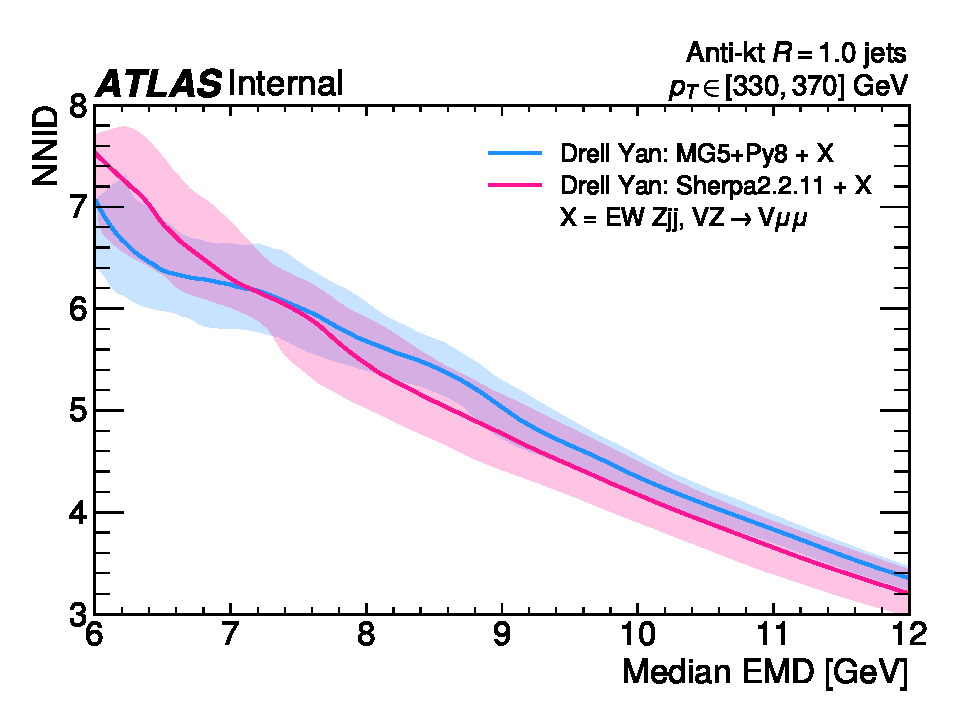
\includegraphics[width=\linewidth, alt={NNID versus median EMD at low EMD scales, comparing MadGraph and Sherpa generators.}]{figures/ch2/gen_meas_nnid_low}
    \label{fig:nnid_low}
  \end{subfigure}
  \hfill
  \begin{subfigure}[b]{0.48\textwidth}
    \centering
    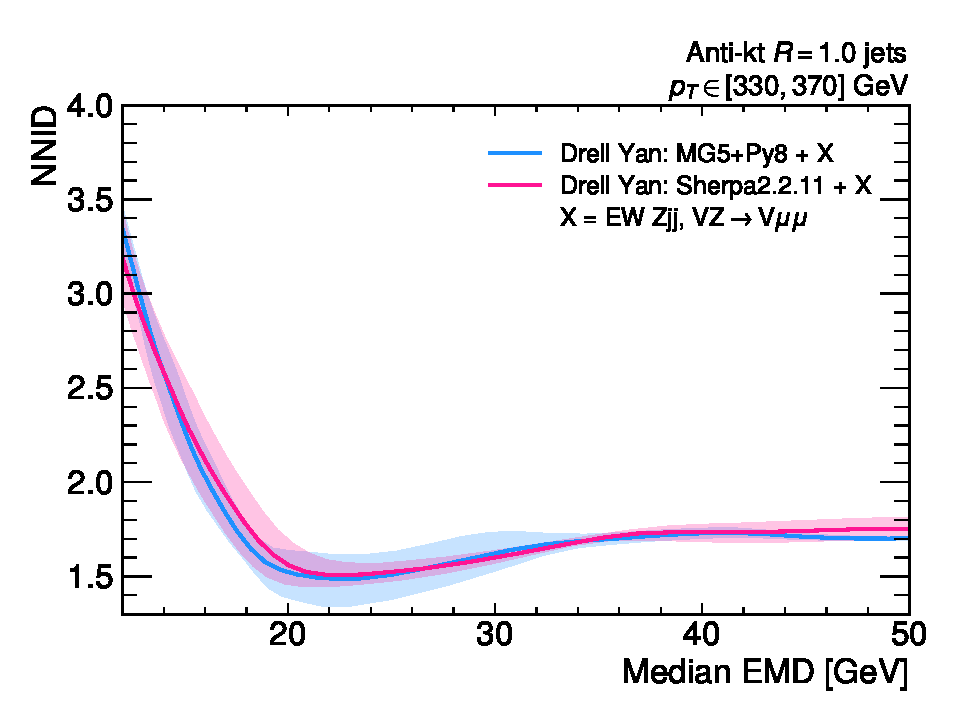
\includegraphics[width=\linewidth, alt={NNID versus median EMD at high EMD scales, comparing MadGraph and Sherpa generators.}]{figures/ch2/gen_meas_nnid_high}
    \label{fig:nnid_high}
  \end{subfigure}
  \caption{Nearest-neighbor intrinsic dimension (NNID) as a function of the median EMD scale, computed at truth level for the \textsc{MadGraph} (blue) and \textsc{Sherpa} (pink) event generators used in Chapter~\ref{ch:zjets}. The two views show the same curve over different ranges of the EMD axis to resolve fine structure. General agreement within uncertainties is observed.}
  \label{fig:nnid_generators}
\end{figure}

The first measurement of the intrinsic dimensionality of jet data is presented in \Cref{sec:zjets-results-id}.
It represents a somewhat different approach to jet physics, in which the focus is on asking basic questions about the experimental data ``as data'' and then evaluating the ability of QCD and the Standard Model to reproduce the answers.
This experimentally driven approach to measurements complements the typical approach of targeting observables due to their connection to the underlying theory.
